\chapter{Électrostatique~: champ et théorème de Gauss}\label{ch:b1:electrostatics-gauss}

Frottez un ballon sur un pull et il se colle au mur~; peignez des cheveux
secs et le peigne dévie un mince filet d'eau. Derrière l'un et l'autre, il y
a la force entre \omterm{def:b1:electrostatics-gauss:charge}{charges électriques} au repos, la \omterm{thm:b1:electrostatics-gauss:coulomb}{loi de Coulomb} --- une loi
en carré inverse comme la \omterm{def:b1:central-forces:gravitation}{gravitation}, mais $10^{36}$ fois plus intense entre
deux protons et de deux signes, si bien que la matière est neutre avec une
précision fantastique et que les effets résiduels s'appellent chimie,
matériaux et foudre. Ce chapitre construit le concept qui rend la loi
maniable, le \omterm{def:b1:electrostatics-gauss:field}{champ électrique}, montre comment lire un champ sur ses
symétries, et démontre le théorème unique qui calcule en trois lignes le
champ des distributions symétriques~: le \omterm{thm:b1:electrostatics-gauss:gauss}{théorème de Gauss}. Son jumeau
gravitationnel vient en prime à la fin.

\begin{omfigure}
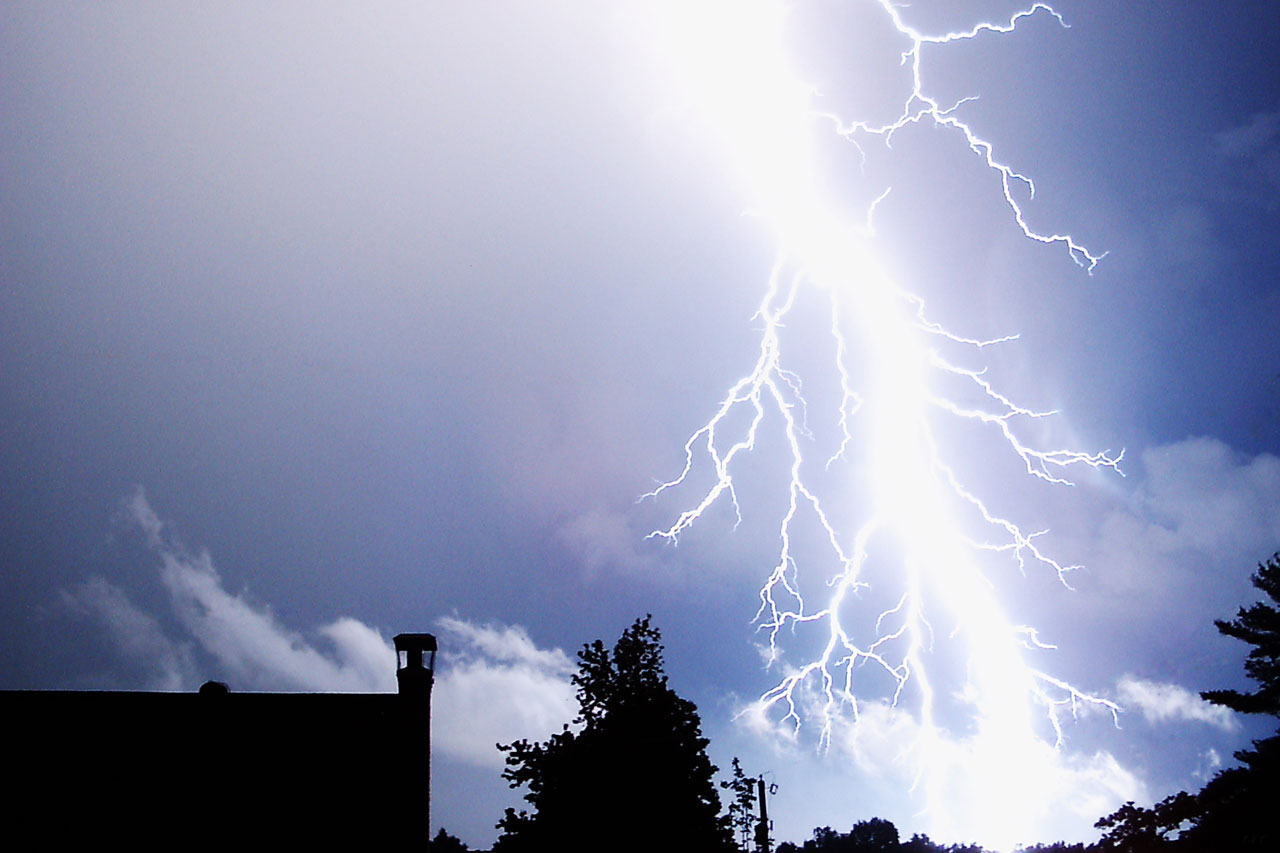
\includegraphics[width=0.50\linewidth]{images/book3/lightning-strike.jpg}

{\small Un éclair nuage--sol~: des dizaines de coulombs amenés au sol en quelques arcs de cent kiloampères --- la Terre électrique du problème du week-end.}
\end{omfigure}

\section{Les charges et la loi de Coulomb}

\begin{definition}[Charge électrique]\label{def:b1:electrostatics-gauss:charge}
\index{charge électrique}\index{charge élémentaire}\index{densité de charge}
La \emph{charge électrique} $q$ (le coulomb, \unit{C}) est une propriété de la
matière, des deux signes~; elle se conserve (la charge totale d'un système
isolé ne change jamais) et elle est quantifiée en multiples de la \emph{charge
élémentaire} $e = \qty{1.602e-19}{C}$ (proton $+e$, électron $-e$). Une
distribution macroscopique se décrit par une \emph{densité de charge}~:
linéique $\lambda$ (\unit{C/m}), surfacique $\sigma$ (\unit{C/m^2}) ou
volumique $\rho$ (\unit{C/m^3}), de sorte qu'un petit élément porte
$\dd q = \lambda\,\dd l$, $\sigma\,\dd S$ ou $\rho\,\dd\tau$.
\end{definition}

\begin{theorem}[Loi de Coulomb]\label{thm:b1:electrostatics-gauss:coulomb}
\index{loi de Coulomb}\index{permittivité du vide}
Deux charges ponctuelles $q_1$ en $M_1$ et $q_2$ en $M_2$, au repos dans le
vide, exercent l'une sur l'autre les forces
\[
\vect F_{1 \to 2} = \frac{q_1q_2}{4\pi\varepsilon_0\,r^2}\,\vect e_{12} = -\vect F_{2 \to 1},
\qquad r = M_1M_2,\quad \vect e_{12} = \frac{\vect{M_1M_2}}{r},
\]
répulsives entre charges de même signe, attractives entre charges opposées, où
$\varepsilon_0 = \qty{8.854e-12}{F/m}$ est la \emph{\omterm{thm:b1:electrostatics-gauss:coulomb}{permittivité du vide}}, c'est-à-dire
$1/4\pi\varepsilon_0 = \qty{8.99e9}{N.m^2/C^2}$. Les forces de plusieurs charges
s'ajoutent (superposition).
\end{theorem}
\admitted

\begin{example}[Quelle intensité]\label{ex:b1:electrostatics-gauss:strong}
Deux protons distants de \qty{1}{fm} se repoussent avec $8.99 \times 10^9 \times (1.6 \times
10^{-19})^2/10^{-30} = \qty{230}{N}$ --- le poids d'un enfant, entre deux
particules de $10^{-27}$~kg~; leur attraction gravitationnelle est
$10^{36}$ fois plus faible. Deux grammes d'électrons à un bout d'une pièce et
les protons correspondants à l'autre s'attireraient avec $10^{25}$~N. La
matière est neutre parce qu'elle n'a pas le choix~: tout déséquilibre est
corrigé par des forces qu'aucune structure ne peut supporter.
\end{example}

\section{Le champ électrique}

\begin{definition}[Champ électrostatique]\label{def:b1:electrostatics-gauss:field}
\index{champ électrique}\index{ligne de champ}
Une distribution de charges au repos crée en tout point $M$ de l'espace un
\emph{champ électrique} $\vect E(M)$, défini par la force qu'il exerce sur une
charge d'épreuve $q$ placée en $M$~: $\vect F = q\vect E(M)$ (\unit{V/m} $=$
\unit{N/C}). Une charge ponctuelle $q_1$ en $O$ crée
\[
\vect E(M) = \frac{q_1}{4\pi\varepsilon_0 r^2}\,\vect e_r , \qquad r = OM ,
\]
radial, dirigé vers l'extérieur si $q_1 > 0$~; une distribution crée la somme
vectorielle des champs de ses éléments. Une \emph{ligne de champ} est une
courbe tangente en chaque point à $\vect E$, orientée dans son sens.
\end{definition}

\begin{proposition}[Lire une carte de champ]\label{prop:b1:electrostatics-gauss:lines}
Les \omterm{def:b1:electrostatics-gauss:field}{lignes de champ} partent des charges positives et aboutissent aux charges
négatives (ou à l'infini)~; elles ne se croisent jamais (le champ a une valeur
unique), et elles se resserrent là où le champ est intense. En présence de deux
charges, le nombre de lignes tracées à partir de chacune est proportionnel à sa charge.
\end{proposition}

\begin{omfigure}
\begin{tikzpicture}[font=\small, x=1cm, y=1cm, >=Stealth]
  % dipole: arcs through (-1,0) and (1,0), centre (0,c)
  \begin{scope}[scale=1.4]
    \foreach \c in {0.1, 0.55, 1.6} {
      \draw[omDef, thick, postaction={decorate, decoration={markings, mark=at position 0.5 with {\arrow{>}}}}]
        let \n1 = {sqrt(1+\c*\c)} in
        (-1,0) arc[start angle={180+atan2(\c,1)}, end angle={360-atan2(\c,1)}, radius=\n1 cm];
      \draw[omDef, thick, postaction={decorate, decoration={markings, mark=at position 0.5 with {\arrow{>}}}}]
        let \n1 = {sqrt(1+\c*\c)} in
        (-1,0) arc[start angle={180-atan2(\c,1)}, end angle={atan2(\c,1)}, radius=\n1 cm];
    }
    \draw[omDef, thick, postaction={decorate, decoration={markings, mark=at position 0.5 with {\arrow{>}}}}] (-1,0) -- (1,0);
    \draw[omDef, thick, postaction={decorate, decoration={markings, mark=at position 0.6 with {\arrow{>}}}}] (-2.6,0) -- (-1,0);
    \draw[omDef, thick, postaction={decorate, decoration={markings, mark=at position 0.4 with {\arrow{>}}}}] (1,0) -- (2.6,0);
    \fill[omThm] (-1,0) circle (3pt) node[below left] {$+q$};
    \fill[omDef] (1,0) circle (3pt) node[below right] {$-q$};
  \end{scope}
  % two like charges
  \begin{scope}[xshift=7.9cm, fl/.style={omThm, thick, postaction={decorate, decoration={markings, mark=at position 0.55 with {\arrow{>}}}}}]
    \foreach \s in {1,-1} {
      % left charge at (-1,0), right charge at (1,0); \s mirrors up/down
      \draw[fl] (-1,0) -- (-3.4,0);
      \draw[fl] (1,0) -- (3.4,0);
      \draw[fl] (-1,0) .. controls (-2.2,{1.2*\s}) .. (-3.2,{2.0*\s});
      \draw[fl] (1,0) .. controls (2.2,{1.2*\s}) .. (3.2,{2.0*\s});
      \draw[fl] (-1,0) .. controls (-1.1,{1.3*\s}) .. (-1.6,{2.9*\s});
      \draw[fl] (1,0) .. controls (1.1,{1.3*\s}) .. (1.6,{2.9*\s});
      \draw[fl] (-1,0) .. controls (-0.2,{0.7*\s}) and (-0.1,{1.6*\s}) .. (-0.3,{2.9*\s});
      \draw[fl] (1,0) .. controls (0.2,{0.7*\s}) and (0.1,{1.6*\s}) .. (0.3,{2.9*\s});
    }
    \draw[fl] (-1,0) -- (-0.08,0);
    \draw[fl] (1,0) -- (0.08,0);
    \fill[omThm] (-1,0) circle (3pt) node[below left] {$+q$};
    \fill[omThm] (1,0) circle (3pt) node[below right] {$+q$};
    \fill (0,0) circle (1.2pt) node[below, font=\footnotesize, yshift=-2pt] {$\vect E = \vect 0$};
  \end{scope}
\end{tikzpicture}

{\small \omterm{def:b1:electrostatics-gauss:field}{Lignes de champ} de deux charges opposées (à gauche) et de deux charges
positives égales (à droite). Les lignes partent du $+$ et aboutissent au $-$
ou à l'infini~; à droite elles se repoussent et le champ s'annule au milieu,
où ne passe aucune ligne.}
\end{omfigure}

\begin{example}[Anneau et segment par sommation directe]\label{ex:b1:electrostatics-gauss:ring}
Sur l'axe d'un anneau de rayon $R$ portant uniformément $Q$, à la distance
$z$ de son centre, chaque élément $\dd q$ contribue pour $\dd q/4\pi\varepsilon_0(R^2 +
z^2)$ selon la droite qui le joint à $M$~; les composantes perpendiculaires
à l'axe se compensent deux à deux et les composantes axiales s'ajoutent avec
le facteur $z/\sqrt{R^2 + z^2}$~:
\[
E_z = \frac{Qz}{4\pi\varepsilon_0(R^2 + z^2)^{3/2}} ,
\]
nul au centre, maximal en $z = R/\sqrt2$, et égal à $Q/4\pi\varepsilon_0z^2$ au
loin. Un disque uniformément chargé est un empilement d'anneaux (\cref{pb:b1:electrostatics-gauss:1}).
La sommation directe fonctionne dès que la géométrie permet l'intégrale~; tout
le reste du chapitre consiste à l'éviter.
\end{example}

\section{Symétries et invariances}

\begin{proposition}[Principe de symétrie]\label{prop:b1:electrostatics-gauss:symmetry}
\index{symétrie (d'un champ)}\index{plan de symétrie}\index{plan d'antisymétrie}
Le champ possède les symétries de ses sources. Si un plan $\Pi$ est un
\emph{\omterm{prop:b1:electrostatics-gauss:symmetry}{plan de symétrie}} de la distribution de charges (l'image miroir de la
distribution est elle-même), alors en tout point de $\Pi$ le champ est
\emph{contenu} dans $\Pi$~; si $\Pi$ est un \emph{\omterm{prop:b1:electrostatics-gauss:symmetry}{plan d'antisymétrie}}
(l'image miroir est la distribution dont toutes les charges sont changées de
signe), le champ en un point de $\Pi$ est \emph{perpendiculaire} à $\Pi$. Si
la distribution est invariante par une translation ou une rotation, le champ
l'est aussi~: ses composantes ne dépendent pas de la coordonnée correspondante.
\end{proposition}

\begin{proof}
$\vect E$ est une somme de termes $\dd q\,\vect e/4\pi\varepsilon_0r^2$~; l'image
miroir de la somme est la somme des images, et l'image du champ d'une
distribution est le champ de la distribution image (un vecteur construit à
partir des positions et des charges se transforme comme les positions). Sur un
\omterm{prop:b1:electrostatics-gauss:symmetry}{plan de symétrie}, le champ est égal à sa propre image miroir, donc il est
contenu dans le plan~; sur un \omterm{prop:b1:electrostatics-gauss:symmetry}{plan d'antisymétrie}, il est égal à l'opposé de
son image, donc il lui est normal. Pour l'invariance, c'est le même argument
avec une translation ou une rotation.
\end{proof}

\begin{method}[Trouver la forme d'un champ avant de le calculer]\label{meth:b1:electrostatics-gauss:symmetry}
Pour le point $M$ où l'on cherche le champ~: (1) recenser les \omterm{prop:b1:electrostatics-gauss:symmetry}{plans de
symétrie} des sources qui contiennent $M$ --- le champ est porté par leur
intersection~; deux tels plans en fixent la direction. (2) Recenser les
invariances --- elles disent de quelles coordonnées $\vect E$ dépend. Ainsi un
fil infini uniformément chargé donne $\vect E = E(r)\,\vect e_r$ en
\omterm{def:b1:point-kinematics:cylindrical}{coordonnées cylindriques}, une sphère $\vect E = E(r)\,\vect e_r$ en
\omterm{def:b1:point-kinematics:spherical}{coordonnées sphériques}, un plan infini $\vect E = E(z)\,\vect e_z$ avec
$E(-z) = -E(z)$. Ce n'est qu'ensuite que l'on calcule.
\end{method}

\begin{omfigure}
\begin{tikzpicture}[font=\small, x=1cm, y=1cm, >=Stealth]
  % sphere
  \begin{scope}
    \draw[omDef, fill=omDef!15] (0,0) circle (0.9);
    \draw[dashed] (0,0) circle (1.8);
    \foreach \a in {0,45,...,315} \draw[omThm, thick, ->] (\a:1.8) -- ++(\a:0.6);
    \node[font=\footnotesize] at (0,-2.75) {$\vect E = E(r)\,\vect e_r$};
    \node[font=\footnotesize, omDef] at (0,0) {$Q$};
  \end{scope}
  % cylinder / wire
  \begin{scope}[xshift=5.2cm]
    \draw[omDef, very thick] (0,-2.2) -- (0,2.2) node[above, font=\footnotesize] {$\lambda$};
    \draw[dashed] (-1.1,-1.6) rectangle (1.1,1.6);
    \draw[dashed] (0,1.6) ellipse (1.1 and 0.28);
    \draw[dashed] (0,-1.6) ellipse (1.1 and 0.28);
    \foreach \y in {-1.0,-0.3,0.4,1.1} {\draw[omThm, thick, ->] (1.1,\y) -- ++(0.6,0); \draw[omThm, thick, ->] (-1.1,\y) -- ++(-0.6,0);}
    \node[font=\footnotesize] at (0,-2.75) {$\vect E = E(r)\,\vect e_r$ (cylindriques)};
  \end{scope}
  % plane
  \begin{scope}[xshift=10.4cm]
    \draw[omDef, fill=omDef!25] (-1.8,-0.25) -- (1.8,-0.25) -- (2.2,0.25) -- (-1.4,0.25) -- cycle;
    \node[omDef, font=\footnotesize] at (1.9,-0.45) {$\sigma$};
    \draw[dashed] (-0.5,-1.4) rectangle (0.5,1.4);
    \foreach \x in {-1.2,0,1.2} {\draw[omThm, thick, ->] (\x,0.35) -- ++(0,0.9); \draw[omThm, thick, ->] (\x,-0.35) -- ++(0,-0.9);}
    \node[font=\footnotesize] at (0,-2.75) {$\vect E = E(z)\,\vect e_z$, impair en $z$};
  \end{scope}
\end{tikzpicture}

{\small Les trois distributions symétriques du chapitre et les surfaces de
Gauss (en pointillés) qui leur conviennent~: une sphère concentrique, un
cylindre coaxial, une boîte plate à cheval sur le plan. Sur chacune, le champ
est soit normal et de norme uniforme, soit tangent.}
\end{omfigure}

\section{Flux et théorème de Gauss}

\begin{definition}[Flux du champ]\label{def:b1:electrostatics-gauss:flux}
\index{flux du champ électrique}
Découpons une surface $S$ en petits éléments d'aire $\dd S$, chacun muni d'une
normale unitaire $\vect n$ (pour une surface fermée, la normale sortante). Le
\emph{flux} de $\vect E$ à travers $S$ est la somme
\[
\Phi = \sum \vect E\cdot\vect n\,\dd S = \sum E_n\,\dd S \qquad (\unit{V.m}):
\]
la composante normale du champ pondérée par l'aire --- le «~nombre de \omterm{def:b1:electrostatics-gauss:field}{lignes
de champ}~» qui traversent $S$, comptées positivement lorsqu'elles la
traversent dans le sens de $\vect n$.
\end{definition}

\begin{theorem}[Théorème de Gauss]\label{thm:b1:electrostatics-gauss:gauss}
\index{théorème de Gauss}
Le \omterm{def:b1:electrostatics-gauss:flux}{flux} du champ électrostatique à travers toute surface fermée $S$ est égal à
la charge totale enfermée par $S$, divisée par $\varepsilon_0$~:
\[
\Phi_{\text{sortant}} = \frac{Q_{\text{int}}}{\varepsilon_0} .
\]
Les charges extérieures à $S$ ne contribuent pas au \omterm{def:b1:electrostatics-gauss:flux}{flux} (leurs lignes entrent
puis ressortent).
\end{theorem}

\begin{proof}
Pour une charge ponctuelle $q$ au centre d'une sphère de rayon $r$~:
$\vect E$ est radial, de norme $q/4\pi\varepsilon_0r^2$ en tout point de la
sphère, donc $\Phi = E \times 4\pi r^2 = q/\varepsilon_0$ --- indépendant de $r$,
parce que le champ décroît en $1/r^2$ exactement comme l'aire croît. Que la
même chose vaille pour toute surface fermée entourant $q$ (le \omterm{def:b1:electrostatics-gauss:flux}{flux} à travers
un élément de surface ne dépend que de l'angle solide sous lequel il est vu
de $q$), qu'une charge extérieure donne zéro (elle voit deux fois chaque angle
solide, avec des signes opposés), et que les \omterm{def:b1:electrostatics-gauss:flux}{flux} de plusieurs charges
s'ajoutent, est ici admis~; la démonstration complète est dans le volume de
deuxième année.
\end{proof}

\begin{method}[Utiliser le théorème de Gauss]\label{meth:b1:electrostatics-gauss:gauss}
(1) À partir des symétries, écrire la forme de $\vect E$ (direction et
variable dont il dépend). (2) Choisir une \emph{surface de Gauss} fermée
passant par le point $M$, sur laquelle $\vect E$ est partout soit normal et de
même norme $E(M)$, soit tangent~: le \omterm{def:b1:electrostatics-gauss:flux}{flux} vaut alors $E(M)$ fois l'aire de la
partie normale. (3) Compter la charge intérieure. (4) En tirer $E(M)$. Cela
fonctionne pour les sphères, les cylindres infinis et les plans infinis ---
et pour rien d'autre sans outils supplémentaires.
\end{method}

\begin{proposition}[Les trois champs classiques]\label{prop:b1:electrostatics-gauss:three}
\index{champ d'une sphère chargée}\index{champ d'un fil chargé}\index{champ d'un plan chargé}
\begin{enumerate}
  \item Sphère de rayon $R$, de charge $Q$ répartie uniformément dans son
        volume~: $E(r) = \dfrac{Q}{4\pi\varepsilon_0r^2}$ à l'extérieur ($r > R$) ---
        comme si toute la charge était au centre --- et $E(r) =
        \dfrac{Qr}{4\pi\varepsilon_0R^3}$ à l'intérieur, croissant linéairement
        depuis zéro~; continu en $r = R$. Si la charge n'est portée que par
        la surface, le champ intérieur est nul.
  \item Fil infini de charge linéique $\lambda$~: $E(r) =
        \dfrac{\lambda}{2\pi\varepsilon_0 r}$, radial.
  \item Plan infini de charge surfacique $\sigma$~: $E = \dfrac{\sigma}{2\varepsilon_0}$
        de part et d'autre, normal au plan, dirigé en s'en éloignant si
        $\sigma > 0$, \emph{indépendant de la distance}. À la traversée du
        plan, la composante normale saute de $\sigma/\varepsilon_0$.
\end{enumerate}
\end{proposition}

\begin{proof}
(1) Sphère de rayon $r$~: \omterm{def:b1:electrostatics-gauss:flux}{flux} $4\pi r^2E(r)$~; charge intérieure $Q$ si
$r > R$, $Q(r/R)^3$ si $r < R$. (2) Cylindre de rayon $r$ et de hauteur $h$~:
\omterm{def:b1:electrostatics-gauss:flux}{flux} $2\pi rh\,E(r)$ par la surface latérale, nul par les bases (le champ y
est tangent)~; charge $\lambda h$. (3) Boîte plate de section $S$ à cheval
sur le plan~: \omterm{def:b1:electrostatics-gauss:flux}{flux} $2SE$ par les deux bases (le champ est impair en $z$, donc
les deux comptent positivement), nul par le côté~; charge $\sigma S$.
\end{proof}

\begin{omfigure}
\begin{tikzpicture}
\begin{axis}[omaxis, axis x line=bottom, axis y line=left, width=10cm, height=5.6cm,
    xlabel={$r/R$}, ylabel={$E$ (en unités de $Q/4\pi\varepsilon_0R^2$)},
    xlabel style={at={(axis description cs:0.5,-0.1)}, anchor=north},
    xmin=0, xmax=4, ymin=0, ymax=1.3, xtick={1,2,3}, ytick={0.5,1}, samples=80]
  \addplot[omDef, very thick, domain=0:1] {x} node[pos=0.85, above left, font=\footnotesize] {en volume~: $\propto r$};
  \addplot[omDef, very thick, domain=1:4] {1/x^2} node[pos=0.35, above right, font=\footnotesize] {$\propto 1/r^2$};
  \addplot[omThm, thick, dashed] coordinates {(0,0) (1,0)};
  \addplot[omThm, thick, dashed] coordinates {(1,0) (1,1)};
  \node[omThm, font=\footnotesize, anchor=west] at (axis cs:1.08,0.08) {en surface~: $0$ à l'intérieur};
\end{axis}
\end{tikzpicture}

{\small Le \omterm{prop:b1:electrostatics-gauss:three}{champ d'une sphère chargée} en fonction de la distance à son
centre~: linéaire à l'intérieur et en $1/r^2$ à l'extérieur lorsque la charge
remplit le volume (trait plein)~; nul à l'intérieur et identique à l'extérieur
lorsqu'elle est portée par la surface (pointillés). À l'extérieur, rien ne
distingue la sphère d'une charge ponctuelle placée en son centre.}
\end{omfigure}

\begin{example}[Deux plans~: le condensateur plan]\label{ex:b1:electrostatics-gauss:twoplanes}
\index{condensateur plan!champ}
Deux plans parallèles portant $+\sigma$ et $-\sigma$~: chacun crée
$\sigma/2\varepsilon_0$ en s'en éloignant (en s'en rapprochant pour le plan négatif).
Entre les plans, les deux champs s'ajoutent en $\sigma/\varepsilon_0$, dirigé du
$+$ vers le $-$~; à l'extérieur ils se compensent. Avec $\sigma = \qty{1}{\micro C/m^2}$, $E =
10^{-6}/8.85 \times 10^{-12} = \qty{1.1e5}{V/m}$ entre les plans et zéro
dehors~: le champ d'un condensateur chargé est confiné à son intervalle
(\cref{ch:b1:potential-capacitors}).
\end{example}

\begin{omfigure}
\begin{tikzpicture}[font=\small, x=1cm, y=1cm, >=Stealth]
  \draw[omThm, very thick] (-0.8,-2) -- (-0.8,2) node[above] {$+\sigma$};
  \draw[omDef, very thick] (0.8,-2) -- (0.8,2) node[above] {$-\sigma$};
  % field of + plane (red), of - plane (blue), resultant (black)
  \foreach \y in {-1.4,-0.7,0,0.7,1.4} {
    \draw[omThm, ->] (-0.8,\y) -- ++(0.55,0);
    \draw[omThm, ->] (-0.8,\y) -- ++(-0.55,0);
    \draw[omDef, ->] (0.8,\y) -- ++(-0.55,0);
    \draw[omDef, ->] (0.8,\y) -- ++(0.55,0);
  }
  \node[omThm, font=\footnotesize, anchor=east] at (-1.0,-2.4) {$+\sigma$ seul~: $\sigma/2\varepsilon_0$};
  \node[omDef, font=\footnotesize, anchor=west] at (1.0,-2.4) {$-\sigma$ seul~: $\sigma/2\varepsilon_0$};
  \begin{scope}[xshift=7.2cm]
    \draw[omThm, very thick] (-0.8,-2) -- (-0.8,2) node[above] {$+\sigma$};
    \draw[omDef, very thick] (0.8,-2) -- (0.8,2) node[above] {$-\sigma$};
    \foreach \y in {-1.4,-0.7,0,0.7,1.4} \draw[black, very thick, ->] (-0.75,\y) -- (0.7,\y);
    \node[font=\footnotesize] at (0,-2.4) {total~: $\sigma/\varepsilon_0$ entre les plans, $0$ au-dehors};
  \end{scope}
\end{tikzpicture}

{\small Superposition pour deux nappes opposées. À gauche~: les champs
uniformes de chaque nappe seule (en rouge à partir de la positive, en bleu
vers la négative). À droite~: leur somme, $\sigma/\varepsilon_0$ dans l'intervalle et zéro ailleurs.}
\end{omfigure}

\section{L'analogie gravitationnelle}

\begin{proposition}[Théorème de Gauss pour la gravitation]\label{prop:b1:electrostatics-gauss:gravity}
\index{théorème de Gauss!pour la gravitation}\index{champ de gravitation}
La loi de Newton $\vect F = -Gm_1m_2\,\vect e_{12}/r^2$ a la forme de celle de
Coulomb avec $q \to m$ et $1/4\pi\varepsilon_0 \to -G$. Le \omterm{prop:b1:electrostatics-gauss:gravity}{champ de gravitation}
$\vect g$ (force par unité de masse) obéit donc aux mêmes règles de symétrie
et à
\[
\Phi_{\text{sortant}}(\vect g) = -4\pi G\,M_{\text{int}} .
\]
En particulier, un corps à symétrie sphérique attire les points extérieurs
comme si toute sa masse était en son centre, et le champ à l'intérieur d'une
sphère uniforme de rayon $R$ et de masse $M$ vaut $g(r) = GMr/R^3$, linéaire en $r$.
\end{proposition}

\begin{proof}
On remplace $Q/\varepsilon_0$ par $-4\pi GM$ dans la démonstration de la
\cref{prop:b1:electrostatics-gauss:three}~; le signe moins dit que le \omterm{def:b1:electrostatics-gauss:flux}{flux}
entre (la \omterm{def:b1:central-forces:gravitation}{gravitation} attire).
\end{proof}

\begin{example}[À l'intérieur de la Terre]\label{ex:b1:electrostatics-gauss:earth}
Pour une Terre homogène, $g$ décroîtrait linéairement de \qty{9.8}{m/s^2} en
surface jusqu'à zéro au centre~; une pierre lâchée dans un tunnel traversant
la planète y oscillerait harmoniquement avec la période $2\pi\sqrt{R/g} =
\qty{84}{min}$ --- la période d'un satellite rasant. La Terre réelle a un
noyau dense, et $g$ \emph{croît} en fait jusqu'à \qty{10.7}{m/s^2} à la
frontière noyau--manteau avant de décroître (\cref{pb:b1:electrostatics-gauss:1}).
Newton avait besoin du théorème des coquilles pour appliquer sa loi aux
planètes~; le \omterm{thm:b1:electrostatics-gauss:gauss}{théorème de Gauss} le donne en une ligne.
\end{example}

\section{Exercices}

\begin{exercise}[$\star$]\label{exo:b1:electrostatics-gauss:1}
Force électrique et force gravitationnelle entre deux protons distants de
\qty{2.0}{fm}~; leur rapport. Pourquoi, alors, les noyaux tiennent-ils~?
\end{exercise}

\begin{exercise}[$\star$]\label{exo:b1:electrostatics-gauss:2}
Champ à \qty{1.0}{m} d'une charge ponctuelle de \qty{1.0}{\micro C}. La
surface de la Terre porte un champ de \qty{100}{V/m} dirigé vers le bas~:
signe et valeur de la charge de la Terre, assimilée à une sphère de rayon \qty{6370}{km}.
\end{exercise}

\begin{exercise}[$\star$]\label{exo:b1:electrostatics-gauss:3}
Deux charges $+q$ en $x = \pm a$ sur l'axe $x$. Champ sur l'axe $x$ pour
$|x| > a$ et sur l'axe $y$~; montrer que, sur l'axe $y$, $E_y$ est maximal en
$y = a/\sqrt2$. Esquisser les lignes près de l'origine.
\end{exercise}

\begin{exercise}[$\star$]\label{exo:b1:electrostatics-gauss:4}
Charges $+2q$ en $x = 0$ et $-q$ en $x = a$. En quel point de l'axe $x$ le
champ s'annule-t-il~? Combien de \omterm{def:b1:electrostatics-gauss:field}{lignes de champ} partent de $+2q$ pour chacune
qui arrive sur $-q$, et où vont les autres~?
\end{exercise}

\begin{exercise}[$\star\star$]\label{exo:b1:electrostatics-gauss:5}
Un disque de rayon $R$ porte $\sigma$ uniformément. À partir du résultat de
l'anneau, montrer que sur son axe $E_z = \dfrac{\sigma}{2\varepsilon_0}\Bigl(1 - \dfrac{z}{\sqrt{z^2 +
R^2}}\Bigr)$ pour $z > 0$~; vérifier les deux limites $z \ll R$ et $z \gg R$.
\end{exercise}

\begin{exercise}[$\star\star$]\label{exo:b1:electrostatics-gauss:6}
Un noyau d'or ($Z = 79$, $R = \qty{7.0}{fm}$) assimilé à une sphère
uniformément chargée~: champ à sa surface, en $R/2$, à \qty{1}{pm}. Comparer
au champ disruptif de l'air, \qty{3e6}{V/m}.
\end{exercise}

\begin{exercise}[$\star\star$]\label{exo:b1:electrostatics-gauss:7}
Champ d'un fil infini par le \omterm{thm:b1:electrostatics-gauss:gauss}{théorème de Gauss}. Pour un conducteur haute
tension de rayon \qty{1.0}{cm}~: charge linéique pour laquelle le champ à sa
surface atteint la valeur disruptive \qty{3e6}{V/m} (seuil de l'effet
couronne). Champ à \qty{5}{m} dans ce cas.
\end{exercise}

\begin{exercise}[$\star\star$]\label{exo:b1:electrostatics-gauss:8}
Deux plaques parallèles d'aire \qty{1.0}{m^2} portent $\pm\qty{1.0}{\micro C}$.
Champ entre elles~; force sur une plaque (le champ qui agit sur elle est celui
de l'autre plaque seulement --- pourquoi~?)~; pression sur les plaques.
\end{exercise}

\begin{exercise}[$\star\star$]\label{exo:b1:electrostatics-gauss:9}
Câble coaxial~: âme de rayon $a$ portant $+\lambda$, \omterm{def:b1:rays-reflection-refraction:fiber}{gaine} extérieure de rayon
$b$ portant $-\lambda$. Champ dans les trois régions par le \omterm{thm:b1:electrostatics-gauss:gauss}{théorème de Gauss}.
Pour $a = \qty{0.5}{mm}$, $b = \qty{2.5}{mm}$, $\lambda = \qty{10}{nC/m}$~:
champ à la surface de l'âme.
\end{exercise}

\begin{exercise}[$\star\star\star$]\label{exo:b1:electrostatics-gauss:10}
Une coquille sphérique épaisse $R_1 < r < R_2$ porte $Q$ uniformément dans son
volume. Champ dans les trois régions~; vérifier la continuité en $R_1$ et
$R_2$~; où est-il maximal~? Esquisser $E(r)$. Une charge positive placée dans
la cavité~: quelle force subit-elle~?
\end{exercise}

\begin{exercise}[$\star\star\star$]\label{exo:b1:electrostatics-gauss:11}
\emph{La \omterm{def:b1:central-forces:gravitation}{gravitation} à l'intérieur de la Terre.} Noyau~: rayon \qty{3480}{km},
masse volumique \qty{11000}{kg/m^3}~; manteau jusqu'à \qty{6370}{km}, masse
volumique \qty{4500}{kg/m^3}. (a) Masse du noyau, du manteau, totale (comparer
à \qty{5.97e24}{kg}). (b) $g$ à la surface et à la frontière noyau--manteau.
(c) Montrer que $g$ croît avec la profondeur dans le manteau si la masse
volumique du manteau est inférieure aux $\tfrac23$ de la masse volumique
moyenne de ce qui est en dessous, et le vérifier.
\end{exercise}

\begin{exercise}[$\star\star\star$]\label{exo:b1:electrostatics-gauss:12}
\emph{L'atome de Thomson.} On modélise l'atome d'hydrogène par une sphère
positive uniforme de charge $+e$ et de rayon $R = \qty{0.10}{nm}$, l'électron
étant libre à l'intérieur. (a) Force sur l'électron à la distance $r$ du
centre. (b) Montrer qu'il oscille harmoniquement et calculer la fréquence
ainsi que la \omterm{prop:b1:wave-propagation:sinusoidal}{longueur d'onde} de la lumière qu'il émettrait. (c) Comparer aux
raies ultraviolettes de l'hydrogène (\qty{122}{nm} et au-dessous) et commenter
ce que le modèle réussit et ce qu'il manque (\cref{ch:b1:quantum-introduction}).
\end{exercise}

\section{Problème~: la Terre électrique}

\begin{problem}[{Problème du week-end --- le champ de beau temps, le nuage
d'orage, l'éclair, et le théorème de Gauss retourné sur la gravitation}]
\label{pb:b1:electrostatics-gauss:1}
Données~: $\varepsilon_0 = \qty{8.85e-12}{F/m}$, $1/4\pi\varepsilon_0 = \qty{8.99e9}{SI}$,
$e = \qty{1.6e-19}{C}$, rayon de la Terre $R_E = \qty{6.37e6}{m}$, surface
$\qty{5.1e14}{m^2}$, $G = \qty{6.67e-11}{SI}$, $M_E = \qty{5.97e24}{kg}$.

\medskip
\noindent\textbf{Partie I --- Le champ de beau temps.}
Par temps clair, le champ au sol vaut $E_0 = \qty{100}{V/m}$ et il est dirigé
\emph{vers le bas}.
\begin{enumerate}
  \item Sens de la force sur un électron libre au sol~; signe de la charge
        de la Terre.
  \item En assimilant la Terre à une sphère uniformément chargée~: sa charge
        totale, par le \omterm{thm:b1:electrostatics-gauss:gauss}{théorème de Gauss}.
  \item Densité surfacique de charge du sol~; nombre d'électrons en excès par
        centimètre carré.
  \item Force sur un grain de poussière de masse \qty{1}{\micro g} portant
        $100$ \omterm{def:b1:electrostatics-gauss:charge}{charges élémentaires}~; comparer à son poids.
  \item Les mesures montrent que le champ tombe à environ \qty{5}{V/m} à
        \qty{10}{km}. Appliquer le \omterm{thm:b1:electrostatics-gauss:gauss}{théorème de Gauss} à une colonne verticale
        de section \qty{1}{m^2} entre le sol et \qty{10}{km}~: signe et
        valeur de la charge que porte l'air par mètre carré.
  \item Densité volumique moyenne de charge de cet air, et nombre
        correspondant de \omterm{def:b1:electrostatics-gauss:charge}{charges élémentaires} par mètre cube. (L'air contient
        environ $10^9$ ions de chaque signe par mètre cube~: quelle fraction
        de déséquilibre cela représente-t-il~?)
  \item L'air a une faible conductivité $\gamma = \qty{2e-14}{S/m}$, de sorte
        qu'une densité de courant $\gamma E_0$ descend. Courant de beau temps
        total sur le globe~; durée qu'il faudrait pour neutraliser la charge
        de la Terre. Conclure.
\end{enumerate}

\medskip
\noindent\textbf{Partie II --- Le nuage d'orage.}
On modélise un nuage d'orage par deux disques horizontaux de rayon $R = \qty{3}{km}$~:
$-Q$ à l'altitude \qty{3}{km}, $+Q$ à \qty{9}{km}, avec $Q = \qty{40}{C}$.
\begin{enumerate}[resume]
  \item Champ sur l'axe d'un anneau de rayon $a$ portant $q$, à la distance
        $z$ de son centre (symétries, puis sommation).
  \item En sommant sur les anneaux, en déduire le champ sur l'axe d'un disque
        de rayon $R$ et de charge surfacique $\sigma$~:
        $E_z = \dfrac{\sigma}{2\varepsilon_0}\Bigl(1 - \dfrac{z}{\sqrt{z^2 + R^2}}\Bigr)$.
  \item Limites $z \ll R$ et $z \gg R$~; interpréter chacune.
  \item Charge surfacique du disque inférieur~; champ qu'il crée au sol, juste
        au-dessous (sens et valeur).
  \item Champ du disque supérieur au même point~; champ résultant au sol sous
        l'orage. Le sol est conducteur et les charges qu'il porte par
        influence doublent à peu près le résultat (admis)~: comparer aux
        \qty{10}{kV/m} mesurés sous les orages et à la valeur de beau temps.
  \item \omterm{def:b1:electrostatics-gauss:flux}{Flux} du champ à travers une surface fermée entourant tout le nuage~;
        puis à travers une surface n'entourant que le disque inférieur.
  \item Champ à mi-distance des deux disques (\qty{6}{km}), et son sens~;
        comparer au champ disruptif de l'air à cette altitude, environ
        \qty{1.5e6}{V/m}.
  \item Si les \qty{40}{C} étaient concentrés dans une sphère de rayon
        \qty{500}{m}~: champ à sa surface. Pourquoi l'amorçage de la foudre
        reste-t-il une question ouverte~?
\end{enumerate}

\medskip
\noindent\textbf{Partie III --- L'arc en retour.}
Un arc en retour amène \qty{5}{C} au sol en \qty{50}{\micro s} par un canal
long de \qty{3}{km}~; on prendra le champ le long du canal égal à
$10^5$~V/m.
\begin{enumerate}[resume]
  \item Courant moyen.
  \item Travail de la force électrique sur la charge transférée~; puissance
        pendant l'arc~; comparer à la consommation moyenne de l'humanité,
        environ \qty{2e13}{W}.
  \item Le canal a un rayon de \qty{2}{cm}~: masse d'air qu'il contient
        ($\rho = \qty{1.2}{kg/m^3}$), et température qu'elle atteindrait si
        toute l'énergie la chauffait à volume constant ($c_V =
        \qty{720}{J/(kg.K)}$). Les températures réelles du canal sont voisines
        de \qty{30000}{K}~: où part le reste~?
  \item Le tonnerre~: retard par kilomètre, et pourquoi le son d'un canal de
        \qty{3}{km} gronde pendant des secondes.
  \item Dans le monde, environ $50$ arcs nuage--sol se produisent chaque
        seconde~: courant qu'ils font descendre~; comparer à la partie~I et
        compléter le tableau du «~circuit global~».
\end{enumerate}

\medskip
\noindent\textbf{Partie IV --- Le \omterm{thm:b1:electrostatics-gauss:gauss}{théorème de Gauss} retourné sur la \omterm{def:b1:central-forces:gravitation}{gravitation}.}
\begin{enumerate}[resume]
  \item Écrire le \omterm{thm:b1:electrostatics-gauss:gauss}{théorème de Gauss} pour le \omterm{prop:b1:electrostatics-gauss:gravity}{champ de gravitation} $\vect g$ et
        justifier la constante par le cas d'une masse ponctuelle.
  \item Terre homogène~: $g(r)$ à l'intérieur~; valeur en $r = R_E/2$.
  \item Terre réelle, noyau de rayon \qty{3480}{km} et de masse volumique
        \qty{11000}{kg/m^3}~: $g$ à la frontière noyau--manteau~; comparer à
        la surface.
  \item Une pierre lâchée dans un tunnel sans frottement traversant une Terre
        homogène~: équation du mouvement, période de l'oscillation, vitesse au
        centre.
  \item Récapituler~: dans chacune des quatre parties, qu'est-ce que le
        \omterm{thm:b1:electrostatics-gauss:gauss}{théorème de Gauss} a remplacé, et quels quatre nombres méritent d'être
        retenus~?
\end{enumerate}
\end{problem}
